\ppageno=15
\ppreviouspageno=14
\plineno=39
\psublineno=1

\newParkoszpage

{\relsize{-1}
\url{http://wbl.klf.uw.edu.pl/13/2/iParkosz.djvu?djvuopts=&page=55&zoom=width&showposition=0.5,0.18}

\url{http://wbl.klf.uw.edu.pl/13/2/iParkosz.djvu?djvuopts=&page=78&zoom=width&showposition=0.5,0.81}
}

\bigskip

\obeylines
\mono



\fullpreviouslines


{
\color{blue}

Tamen 

eciam in suis locis possemus singulas predictas 
}

\plineno=0

\fulllines

litteras seu earum exempla ponere, sicut et ponemus. Non

est enim vicium idem pluries repetere ex causa notandum.

% \def\splitlines{\advance\plineno by 1\psublineno=0\everypar{\advance\psublineno by 1\llap{\textcolor{green}{\the\ppageno-\ifnum\plineno<10 0\fi\the \plineno-\the\psublineno \ }}}}

% \def\newsplitline{\advance\plineno by 1}

\def\splitverse{\advance\plineno by 1\psublineno=0\everypar{\advance\psublineno by 1\llap{\textcolor{green}{\the\ppageno-\ifnum\plineno<10 0\fi\the \plineno-\the\psublineno \ }}\hskip5em}}

% nie działa licznik wierszy?
\def\fullverselines{\everypar{\advance\plineno by 1\llap{\the\ppageno-\ifnum\plineno<10 0\fi\the \plineno \hskip 1.5em}\hskip5em}}


\def\newverse{\advance\plineno by 1\psublineno=0\hskip10em}
\def\newversesubline{\hskip10em}
\def\newverseline{\advance\plineno by 1\psublineno=0}
\def\indentVerse{\hskip10em}

% MUFI SHORT VIRGULA

{

\catcode`\/=13
\def/{{\fontCardo }}



% 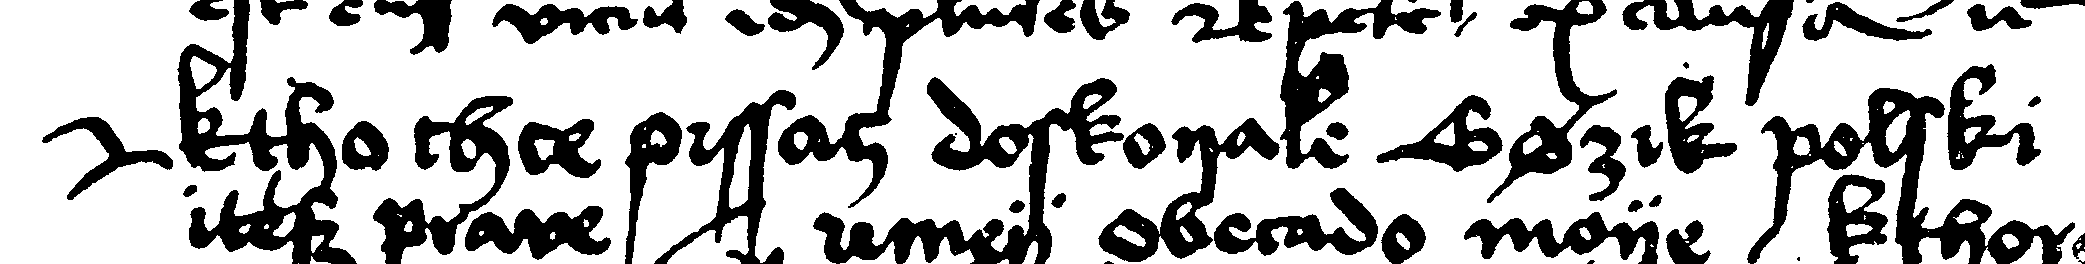
\includegraphics[width=\hsize]{wierszP1m}

\splitverse

Ktho chce piſſaç doſkoɲaɬe

\indentVerse Gøzik poɬſki

% 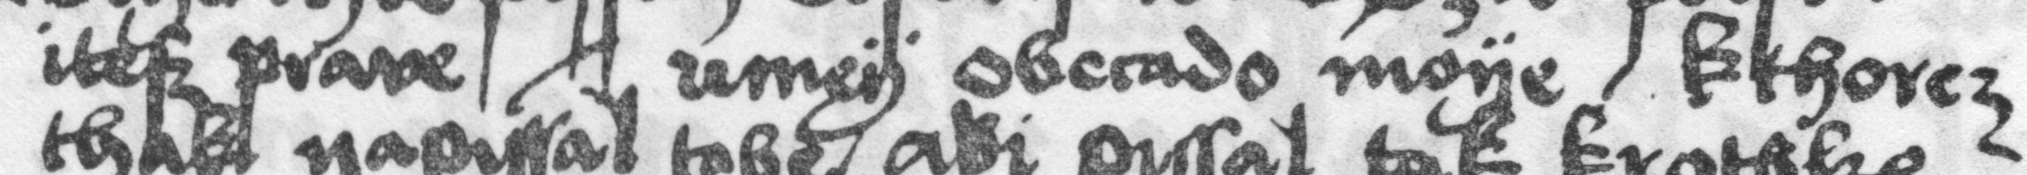
\includegraphics[width=\hsize]{wierszP2}

%\newverse 
\splitverse

itefz prave/


\indentVerse umeij obecado moije/

% http://en.wikipedia.org/wiki/Ezh
% 'LATIN SMALL LETTER EZH' (U+0292)
	

\catcode `\^^M=5
\newtip{85}{Tak w rkp., z pewnością należy czytać \textit{ktorem}, a nie \textit{któreż}, co jednak
nie jest o tyle pewne, że w wyrazach, polskich w traktacie skrótów nie ma.}
\obeylines
kthore\conf{ʒ}{}¹

% 85 Tak w rkp., z pewnością należy czytać Morem, a nie któreś, Co jednak

% nie jest o tyle pewne, że w wyrazach, polskich w traktacie skrótów nie ma.

% 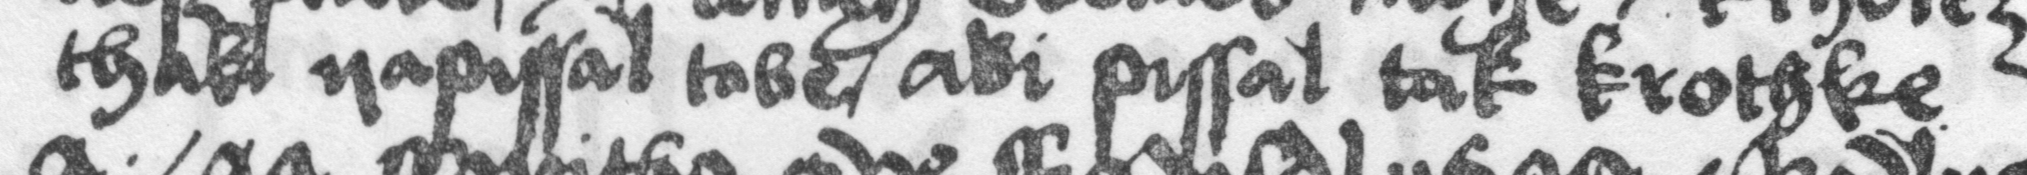
\includegraphics[width=\hsize]{wierszP3}


\splitverse

thak ɲapiſſaƚ toɓe/	

\indentVerse  aɓi piſſaƚ tak krothke 

% 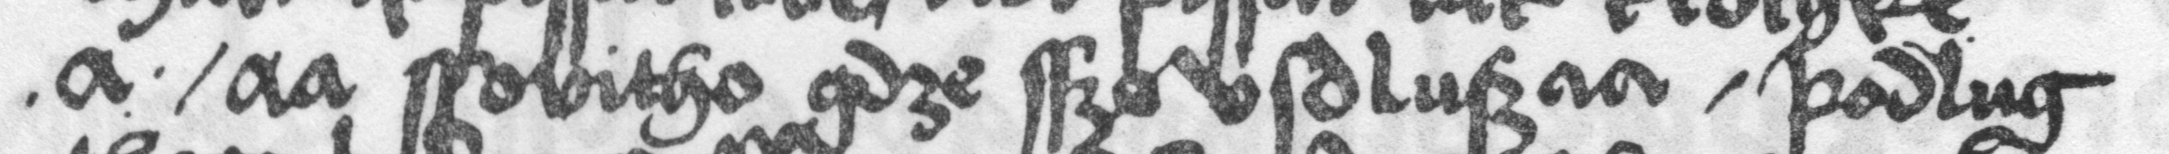
\includegraphics[width=\hsize]{wierszP4}

\splitverse

• a •/

\indentVerse  \textit{aa} ſſovitho ɠdze ſſzø ʋſdƚuſzaa/

\indentVerse  podƚuɠ 

% 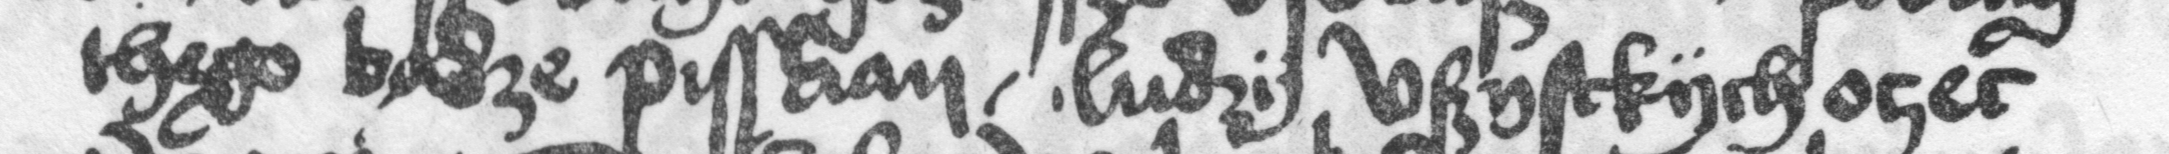
\includegraphics[width=\hsize]{wierszP5}

\splitverse

theɠo bødze piſſaaɲ/

% znika e!!!
\indentVerse ɬudzij ʋſzyſtkijch oçec 

\newpage
% 
\includegraphics[width=\hsize]{wierszP6}

\splitverse

\textit{adaaɱ}/

\indentVerse A theſz gdze • ƀ • bødze gruube/ 

% \newverseline

% 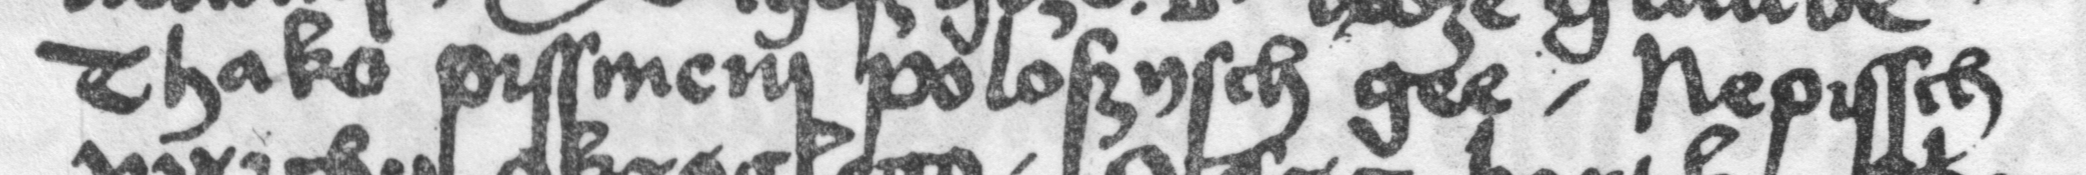
\includegraphics[width=\hsize]{wierszP7}

\splitverse

Thako piſſmeɱ poƚoſzyſch gee/

\newversesubline Nepiſſch 

% 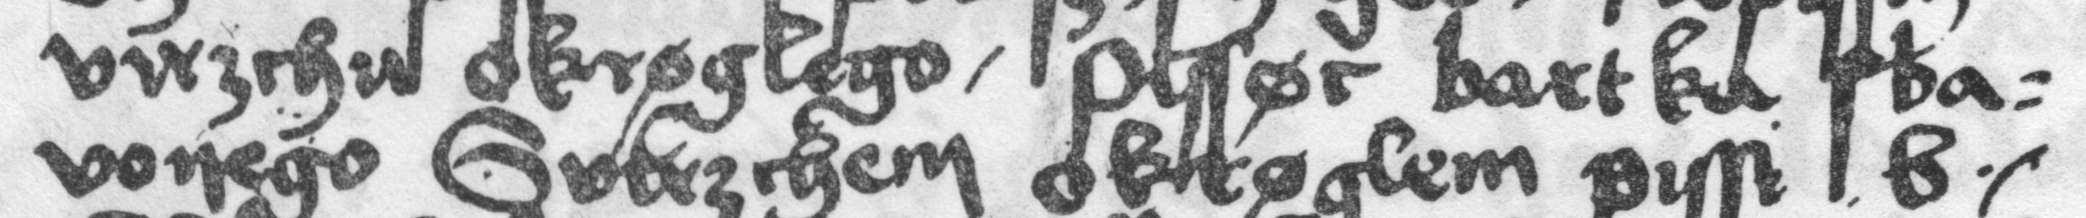
\includegraphics[width=\hsize]{wierszP8}

\splitverse virzchu okrøɠɬeɠo/

% hyphen!!!
\newversesubline Piſſøc \textit{bartka} \textit{\hyphh{ſba}{voɲego}}

% 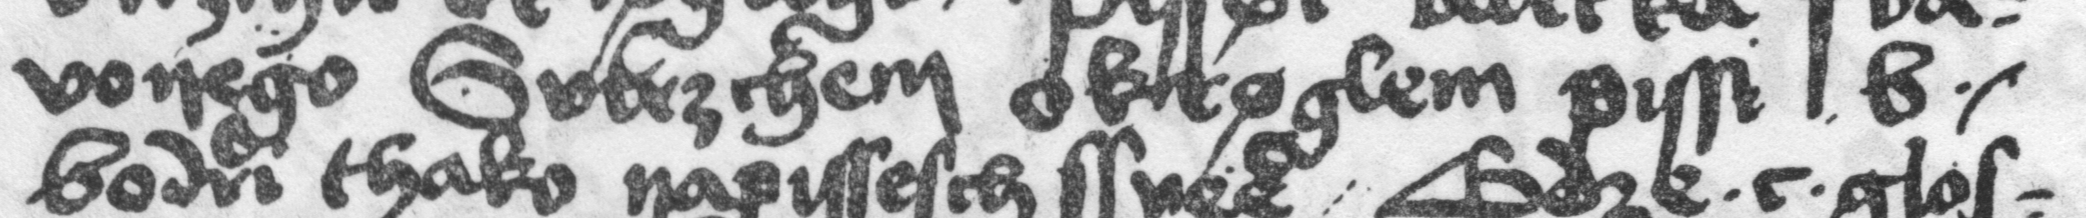
\includegraphics[width=\hsize]{wierszP9}

%\newverseline
\fullverselines

 \textit{\hypht{ſba}{voɲego}} Svirzcheɱ okrøɠɬem piſſi • ɓ •/

% 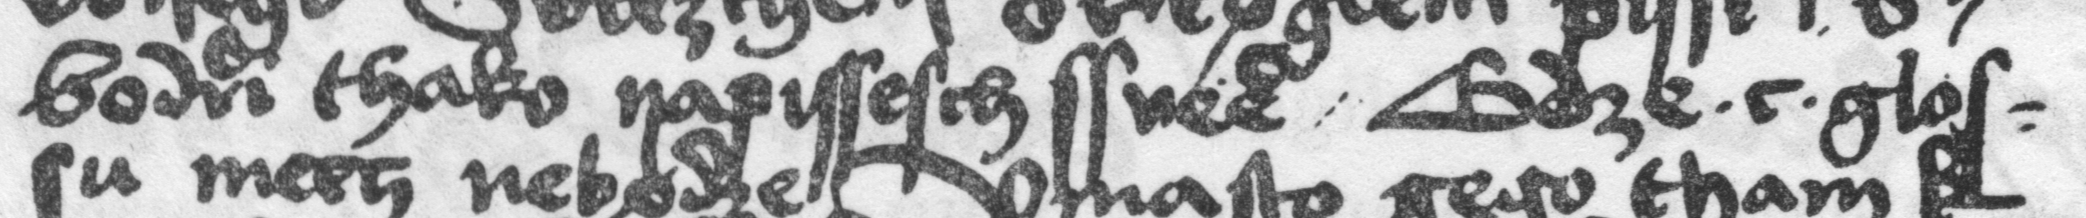
\includegraphics[width=\hsize]{wierszP10}

\plineno=12
\splitverse

\textit{ɓodri} thako ɲapiſſeſch ſſvee/

% zły numer!

\indentVerse Gdze • \textit{c} • \hyphh{gƚoſ}{ſu}

% 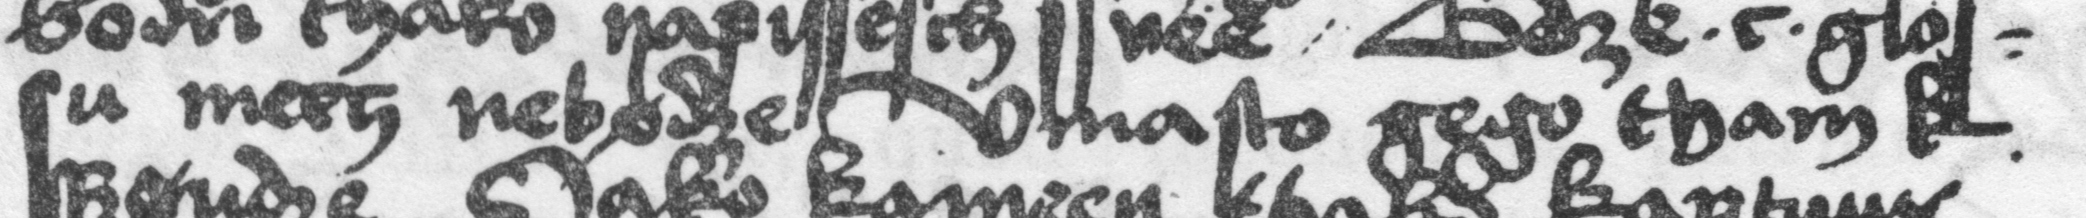
\includegraphics[width=\hsize]{wierszP11}

\splitverse

\hypht{gƚoſ}{ſu} meeç nebødze

\indentVerse Vmaſto geɠo tham \textit{k} 

% 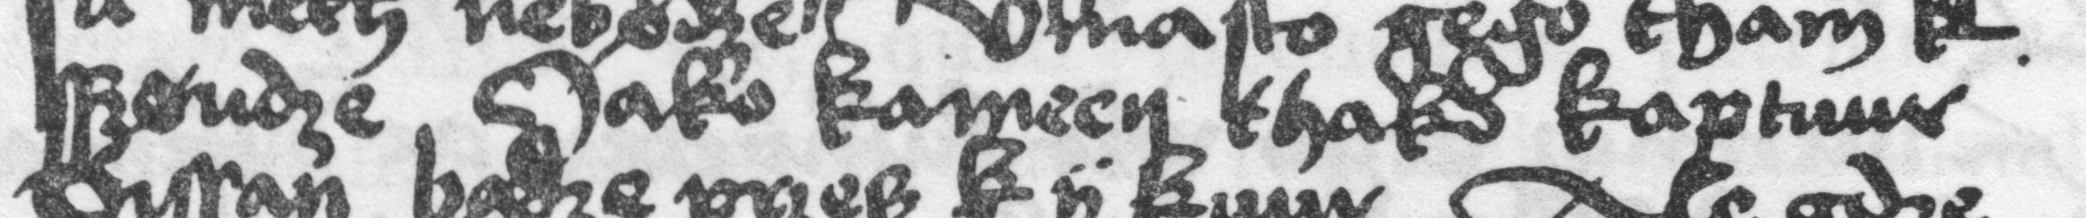
\includegraphics[width=\hsize]{wierszP12}

\splitverse

ſſzøndze

\indentVerse Iako \textit{kameeɲ} thako \textit{kaᵽtuur} 

\newpage
% 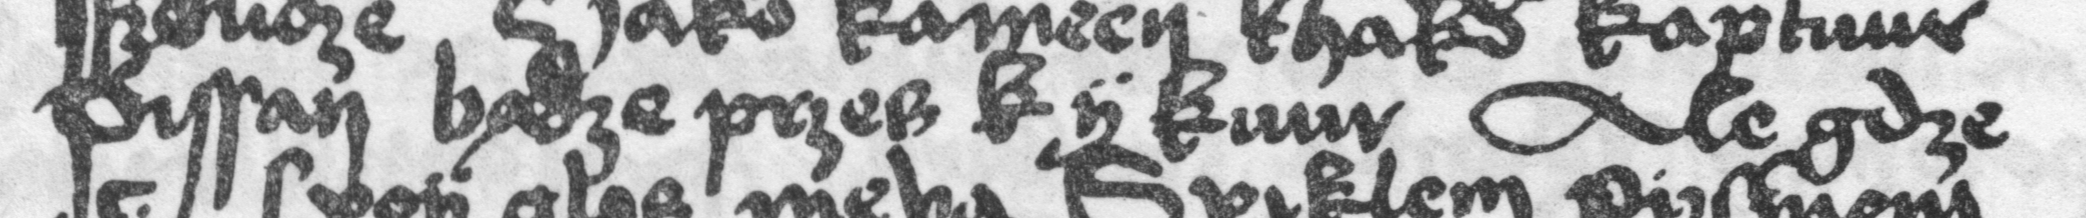
\includegraphics[width=\hsize]{wierszP13}

\splitverse

% brak Ƥ
Ƥiſſaɲ bądze przes \textit{k} ij \textit{kuur}

\indentVerse Aɬe ɠdze 

% 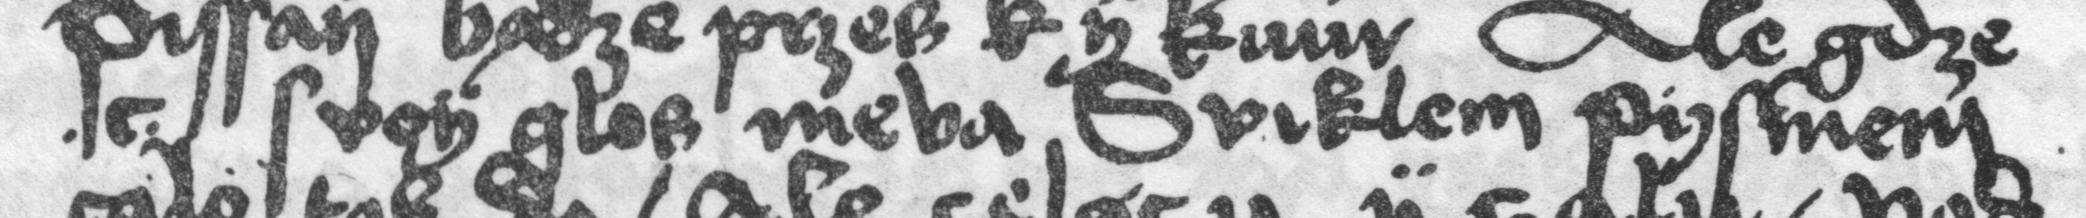
\includegraphics[width=\hsize]{wierszP14}

\splitverse

· \textit{c} • ſvoij ɠƚos meʋa

\indentVerse Svikƚem pijſmeɱ  

% 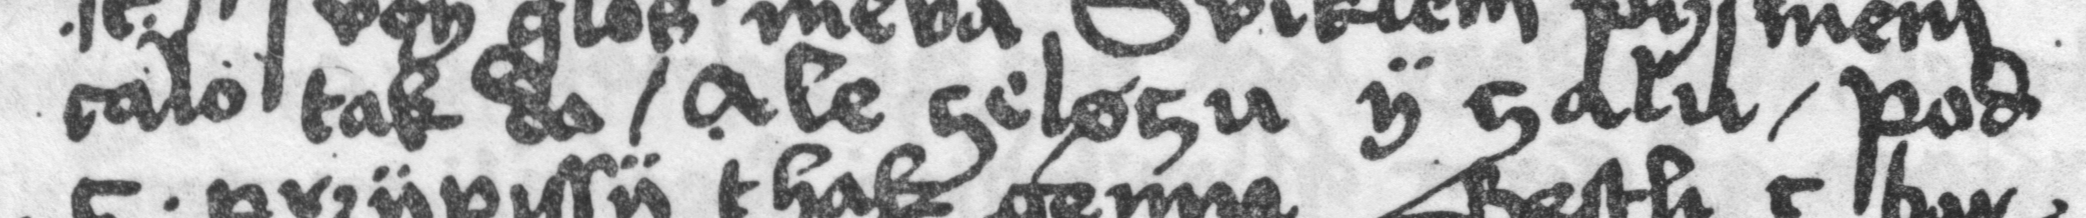
\includegraphics[width=\hsize]{wierszP15}

\splitverse

caƚo tak da/

\indentVerse Aɬe \textit{çeløçu} ij \textit{çalu}/

\indentVerse  pod

% 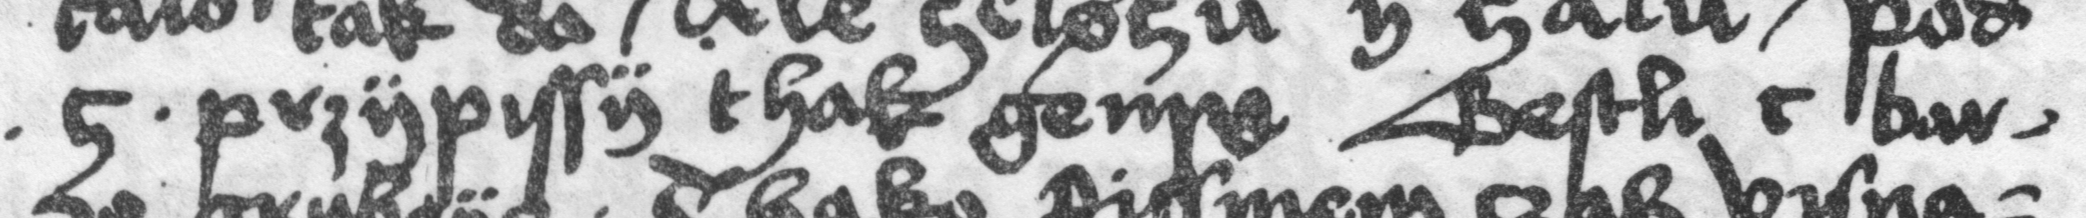
\includegraphics[width=\hsize]{wierszP16}

\splitverse

  • Q • przijpiſſy thak geɱv

\indentVerse Geſtɬi \textit{c} \hyphh{bar}{zo} 

% 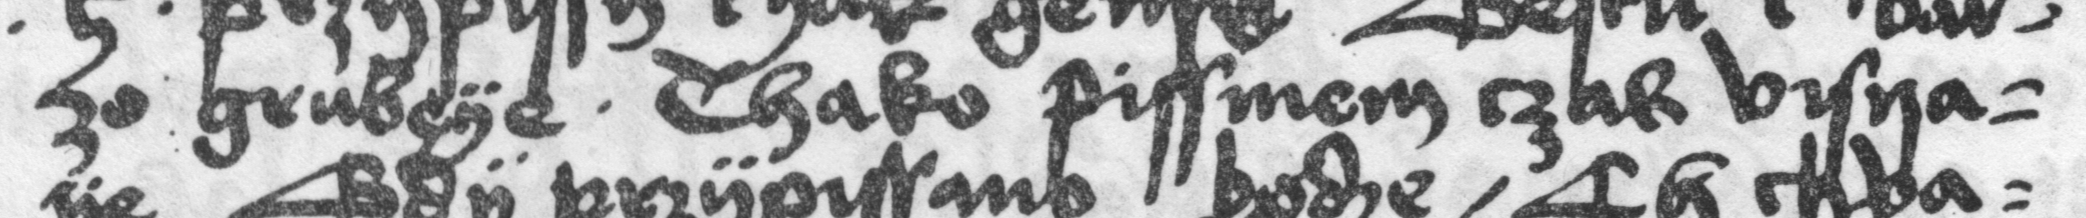
\includegraphics[width=\hsize]{wierszP17}

\newverseline \hypht{bar}{zo} gru6eije.

\indentVerse Thako piſſmem \textit{czas} \hyphh{ʋiſɲa}{ije}

% 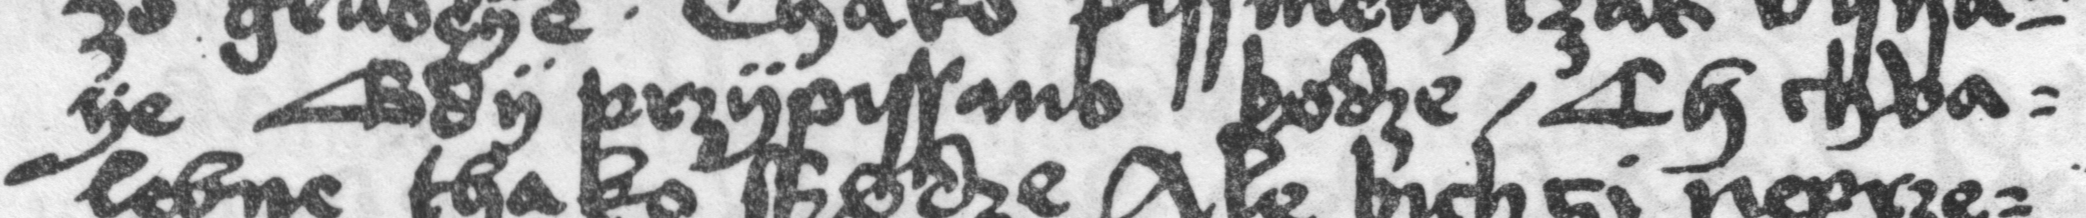
\includegraphics[width=\hsize]{wierszP18}

\newverseline \hypht{ʋiſɲa}{ije} Gdy \add{h} przijpiſſano bødze/

\indentVerse \textit{Ch}  \hyphh{chʋa}{ɬebɲe}

\newpage

% 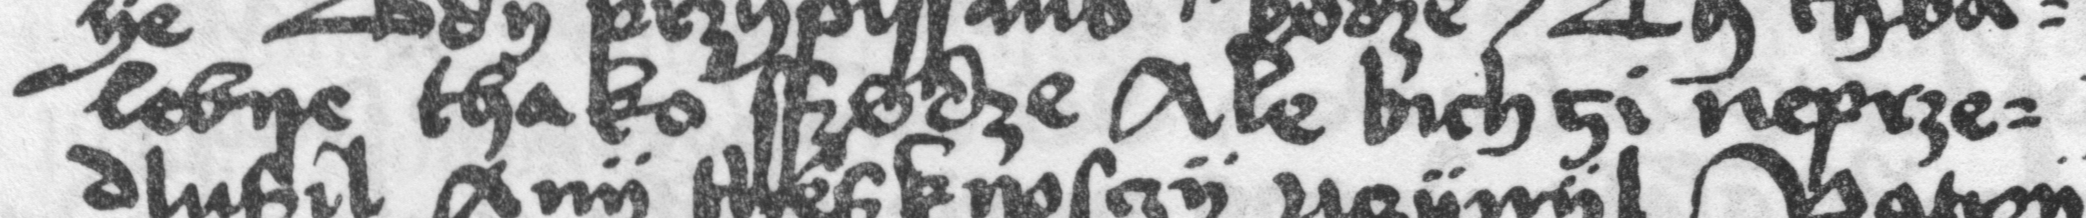
\includegraphics[width=\hsize]{wierszP19}

\splitverse

\hypht{chʋa}{ɬebɲe} thako ſſzødze

\indentVerse Aɬe bich çi \hyphh{neprze}{dƚuſziƚ}

% 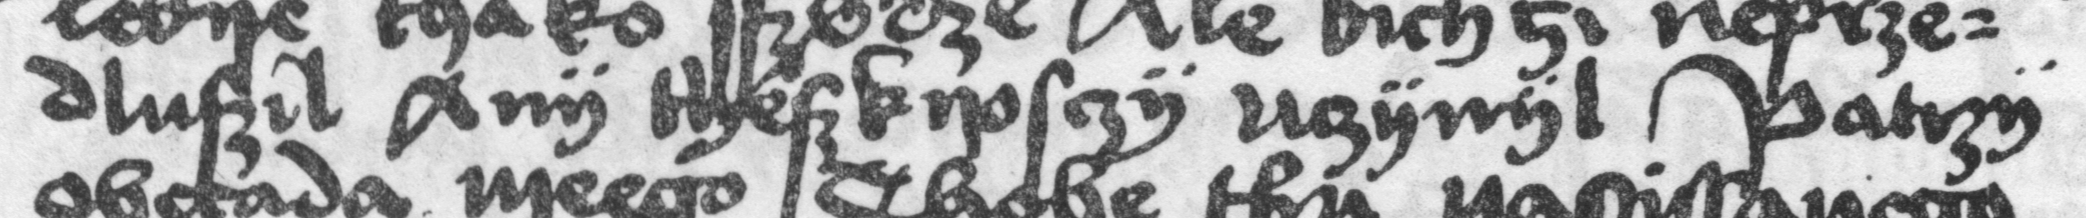
\includegraphics[width=\hsize]{wierszP20}

\splitverse

\hypht{neprze}{dƚuſziƚ}

\indentVerse Anij theſzkɲoſczij uczijnijƚ

\indentVerse Patrzij 

% 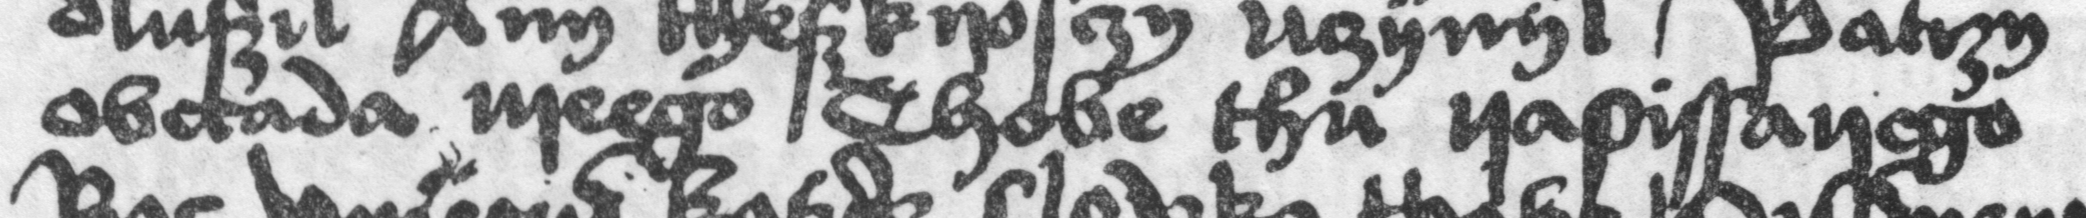
\includegraphics[width=\hsize]{wierszP21}

\splitverse

obecada ɱeego

\indentVerse Thoɓe thu ɲapiſſaɲego 

% 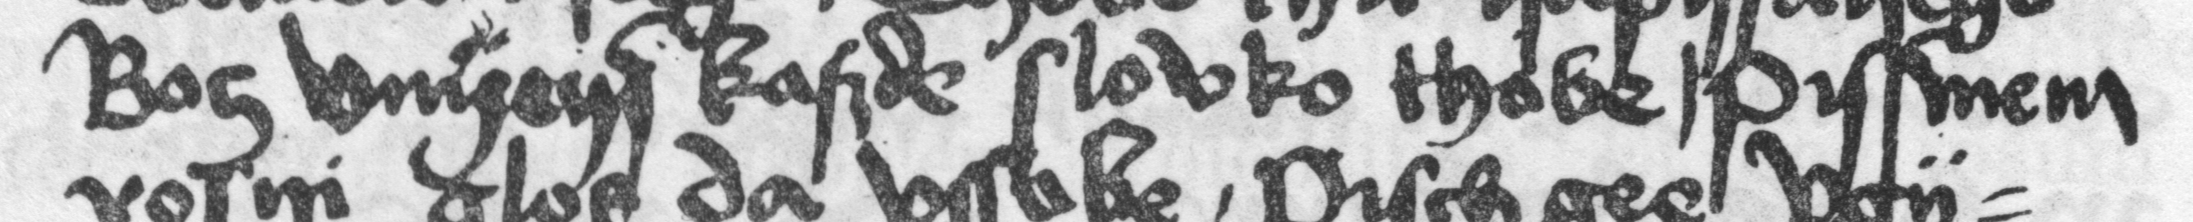
\includegraphics[width=\hsize]{wierszP22}

\splitverse

Boç ʋnye\conf{ɱ}{} kaſzde ſƚoʋko thobe /

\indentVerse Ƥiſſmeɱ 

% 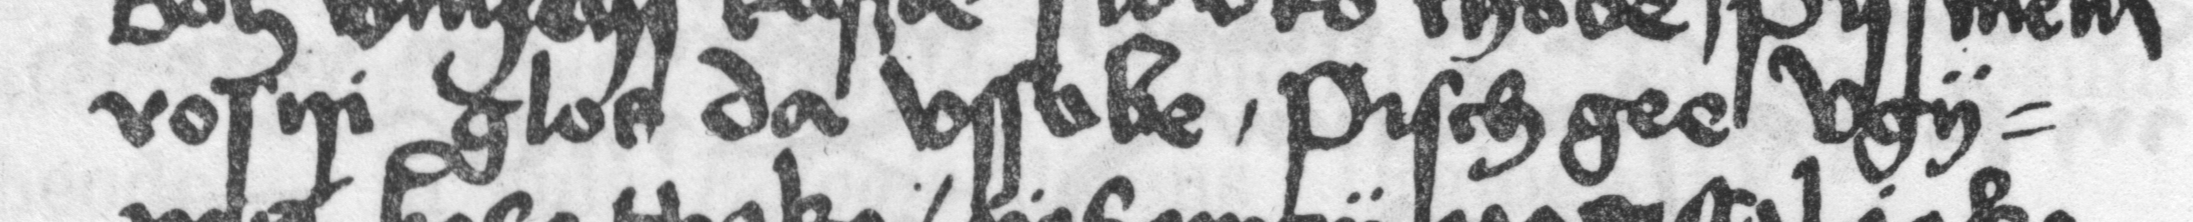
\includegraphics[width=\hsize]{wierszP23}

\splitverse

roſɲi gƚos da ʋſſobe/

\indentVerse  Piſch gee \hyphh{Vgij}{mo}

% 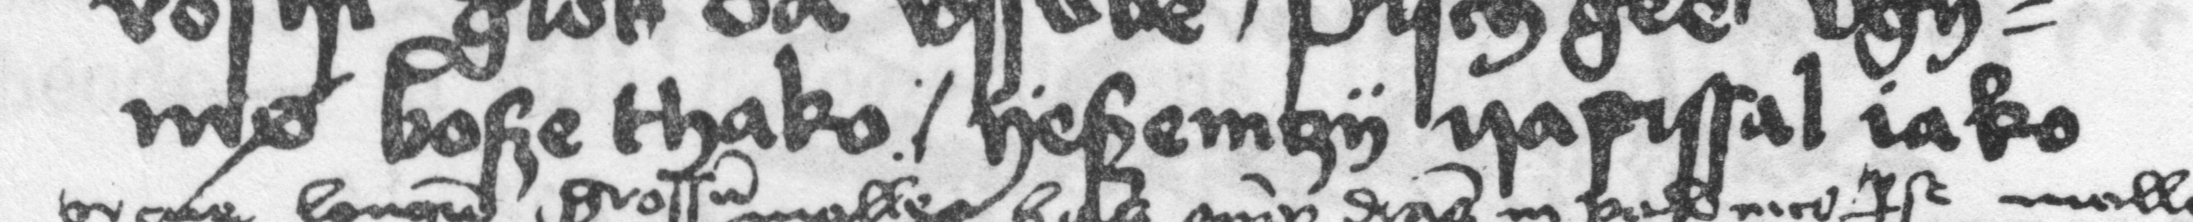
\includegraphics[width=\hsize]{wierszP24}

\splitverse

\hypht{Vgij}{mo} boſze thako/

\catcode `\^^M=5
\newtip{86}{Nie sygnalizujemy pisowni w wielu wypadkach niezgodnej z
  zaleceniami. Cały ten wiersz w pisowni zrekonstruowanej według
  wskazówek Parkosza ogłosił Łoś w Języku Polskim I, 1913, s. 56.}
\obeylines
\indentVerse ijeſzemczij ɲapiſſaƚ iako¹
% •* Nie sygnalizujemy pisowni w wielu wypadkach niezgodnej z zale¬

% ceniami. Cały ten wiersz w pisowni zrekonstruowanej według wskazówek

% Parkosza ogłosił Łoś w Języku Polskim I, 1913, s. 56.

% koniec wiersza!!!

\newpage

\fulllines

% 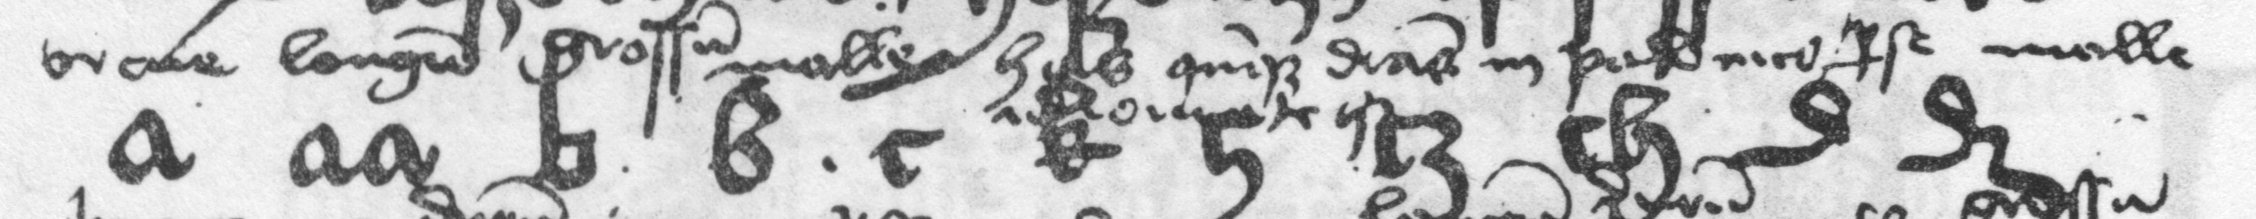
\includegraphics[width=\hsize]{wierszP25-26}


breue longum groſſum molle

a aa ƀ ɓ

c has quinque differencias in Polonico idiomate habet

c k ç cz ch

per ſe molle breue longum durum molle

d dz e ee ff f

% 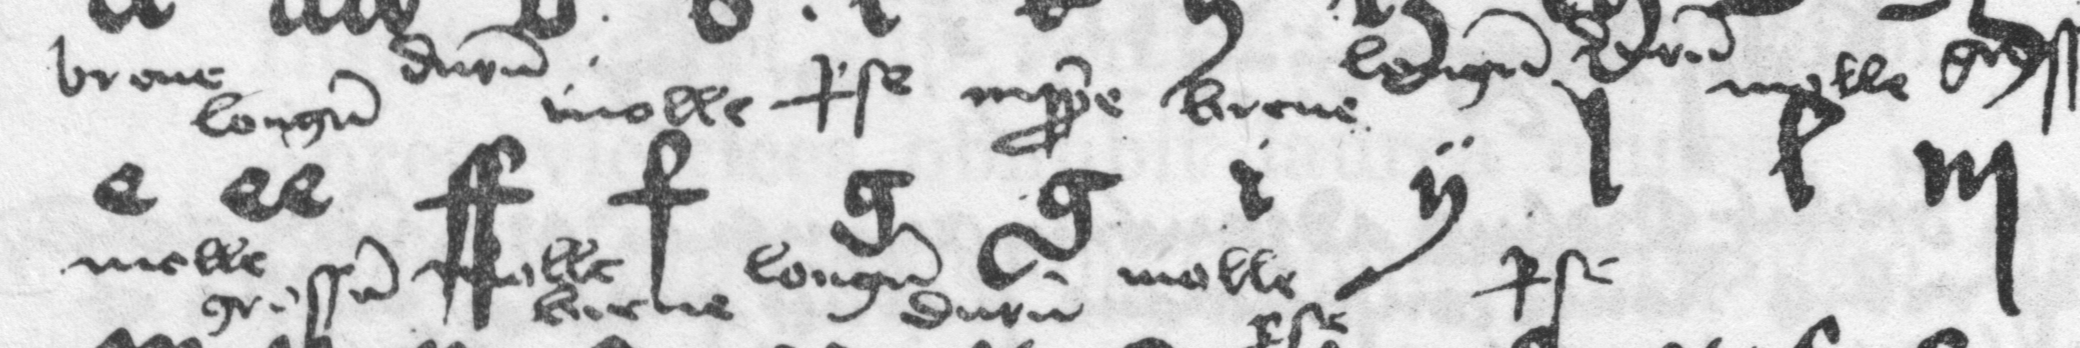
\includegraphics[width=\hsize]{wierszP27-28}

per ſe inproprie breue longum durum molle

\newtip{87}{Winno być: per se \textit{ɠ}, improprie \textit{g}.}
g ɠ¹' i ij ƚ ɬ
% 87	Winno być: per se g, improprie g.

groſſum molle groſſum molle breue longum

ɱ m ɲ n o oo

% 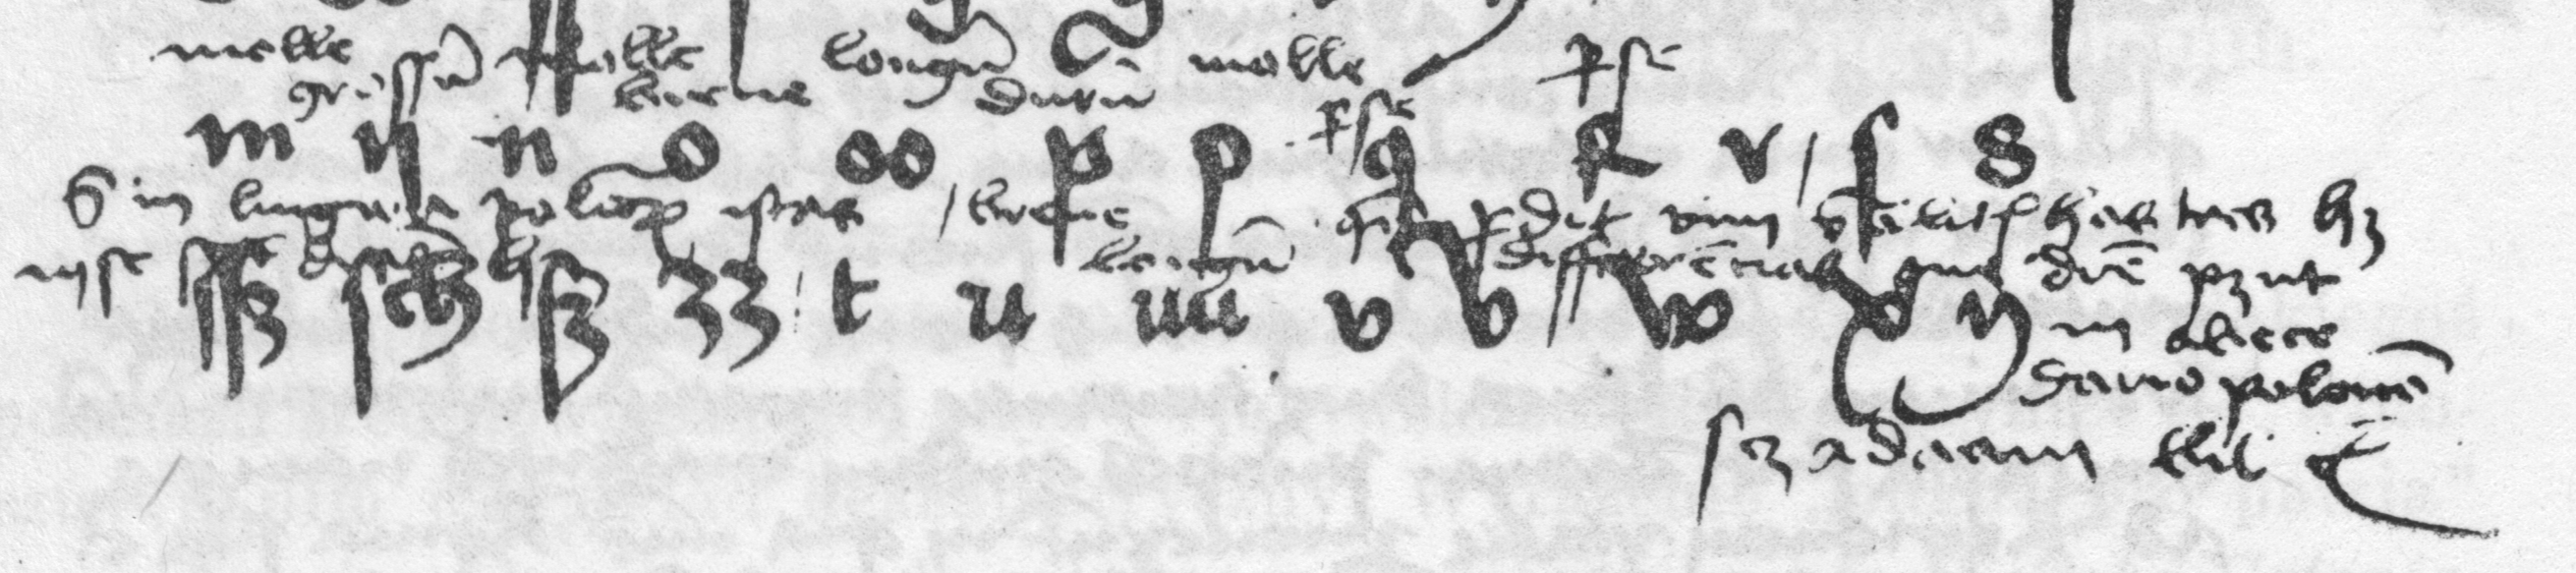
\includegraphics[width=\hsize]{wierszP29-koniec}

durum molle per ſe per ſe

ᵽ ƥ q R r

S in lingua Polonorum iſtas in ſe ſex differencias habet

ſ s 

ſſz ſch ſz zz

breue	longum

% niezlokalizowane w oryginale!!!

t u uu eum perdit vim vocalitatis, has tres habet differencias, 

que differencie patent in abecedario Polonorum, 

ſcilicet adaam ɓiɬ etc.

v ʋ w	x y

}

\endinput



% \fullfines

% \ppreviouspageno=16
% \plineno=0


% \fullpreviouslines


% {
% \color{blue}

% ???


% }




% \endinput


%%%%%%%%%%%%%%%%%%%%%%%%%%%%%%%%%%%%%%%%%%%%%%%%%%%%%%%%%%%%%%%%%%%%%%%%%%%%%%%%%%%%%%%%%%%




\catcode `\^^M=5

  \newtip{48}{Łoś niesłusznie uważa, że \textit{bika} w obu wypadkach
    napisano błędnie zamiast \textit{ƀyka}. Przykłady są bowiem podane
    w~pisowni dotychczasowej dla pokazania jej niewystarczalności do
    zróżnicowania wyrazów \textit{bika} i \textit{byka}.} 

\obeylines






\newcommand{\margin}[1]{\annotatetextBlue{\{#1\}}{zapisy na marginesie}}


% \renewcommand{\over}[1]{\colorbox{blue!10}{\{#1\}}}

\renewcommand{\over}[1]{\annotatetextBlue{\{#1\}}{zapisy nad rządkami}}

% litery i wyrazy dodane, (których w tekście brak)
%\newcommand{\add}[1]{\colorbox{olive!10}{<#1>}}
\newcommand{\add}[1]{\annotatetextOlive{<#1>}{litery i wyrazy dodane, (których w tekście brak)}}

% litery i wyrazy zbędne
% \newcommand{\extra}[1]{\colorbox{magenta!10}{[#1]}}
\newcommand{\extra}[1]{\colorbox{magenta!10}{[#1]}}

% przekreślenia
% MATHEMATICAL LEFT WHITE SQUARE BRACKET' (U+27E6)
% 'MATHEMATICAL RIGHT WHITE SQUARE BRACKET' (U+27E7)
\newcommand{\overstr}[1]{\annotatetextMagenta{⟦#1⟧}{przekreślenia}}



%%% Local Variables: 
%%% mode: latex
%%% TeX-PDF-mode: t
%%% TeX-engine: luatex 
%%% TeX-master: "ParkoszLatin"
%%% default-input-method: "Parkosz-slash"
%%% End: 
